%!TEX TS-program = xelatex
%!TEX encoding = UTF-8 Unicode


\documentclass[11pt]{article}
\usepackage{geometry}
\geometry{letterpaper}

\usepackage{fontspec,xltxtra,xunicode}

\usepackage{xeCJK} % 使用xeCJK宏包
\setCJKmainfont{Yuanti SC Light}   % 设置缺省中文字体

\setmainfont{Yuanti SC Light} % 设置文档默认字体 ,if不指定,使用Tex的默认英文字体
\defaultfontfeatures{Mapping=tex-text}
% \setromanfont{Yuanti SC Light} %设置中文字体
\XeTeXlinebreaklocale “zh”
\XeTeXlinebreakskip = 0pt plus 1pt minus 0.1pt %文章内中文自动换行


\newfontfamily{\H}{SimHei}
\newfontfamily{\E}{Consolas}  %设定新的字体快捷命令
\title{\H 方便网建设意见}
\author{\E Donald}
\date{\E\today}



% a garbage package you don't need except to create examples.
\usepackage{lipsum}

\usepackage{fancyhdr}
\pagestyle{fancy}
% \lhead{This is my name}
\renewcommand{\sectionmark}[1]{\markboth{#1}{}} % set the \leftmark
\lhead{\leftmark}
% \rhead{this is page \thepage}
\rhead{\thepage}
\cfoot{} % center footer
\renewcommand{\headrulewidth}{0.4pt}
\renewcommand{\footrulewidth}{0.4pt}
% clear blank pages
\let\cleardoublepage\clearpage
% page n of m, usage:\thispagestyle{firststyle}
\fancypagestyle{firststyle}
{
	\fancyhf{}
	\fancyfoot[C]{\footnotesize Page \thepage\ of \pageref{LastPage}}
}

% footnote in footer, usage:\fancyfootnotetext{page_num}{this is the footnote}
\newcommand{\fancyfootnotetext}[2]{%
	\fancypagestyle{dingens}{%
		\fancyfoot[LO,RE]{\parbox{\textwidth}{\footnotemark[#1]\footnotesize #2}}%
	}%
	\thispagestyle{dingens}%
}

% prevent floats from passing section
\usepackage[section]{placeins}

% TOC
\usepackage{tocloft}
\renewcommand{\cftsecleader}{\cftdotfill{\cftdotsep}}

% 段落缩进设置
\setlength{\parindent}{2em}
% 首段缩进
\usepackage{indentfirst}

\usepackage{float}

% list style
\usepackage{enumitem}

% caption font size
\usepackage[font=footnotesize,labelfont=bf]{caption}

% preface page
\newenvironment{dedication}
  {\clearpage           % we want a new page
   \thispagestyle{empty}% no header and footer
   % \vspace*{\stretch{1}}% some space at the top 
   \itshape             % the text is in italics
 %  \raggedright          % flush to the right margin
  }
  {\par % end the paragraph
   \vspace{\stretch{3}} % space at bottom is three times that at the top
   \clearpage           % finish off the page
  }

\usepackage[figurename=Fig.]{caption}

% section从新一页开始
\usepackage{titlesec}
\newcommand{\sectionbreak}{\clearpage}

% 目录索引超链接,放在最后
\usepackage[hidelinks]{hyperref}


\begin{document}

% input partials
\begin{titlepage}
	\begin{center}
		
		% Upper part of the page. The '~' is needed because \\
		% only works if a paragraph has started.
		% \includegraphics[width=0.6\textwidth]{graphics/hs}~\\[1cm]
		
		% \textsc{\LARGE EVERTHIS.COM}\\[1.5cm]
		
		% \textsc{\Large Final year project}\\[0.5cm]
		
		% Title
		\rule[1pt]{\textwidth}{2pt}		
		{ \huge \bfseries 方便网建设意见 \\[0.5cm] }		
		\rule[10pt]{\textwidth}{2pt}
		
		% Author and supervisor
		\begin{minipage}{1.0\textwidth}
			\begin{center} \large
				\emph{Author:} 何杰
			\end{center}
		\end{minipage}

		%
		% \begin{minipage}{0.4\textwidth}
		% 	\begin{flushright} \large
		% 		\emph{Supervisor:} \\
		% 		Dr.~Mark \textsc{Brown}
		% 	\end{flushright}
		% \end{minipage}
		% 

		\vfill

		% Bottom of the page
		{\large \today}
		
	\end{center}

\end{titlepage}

% in two-side books, uncomment the line below. otherwise, comment it.
%\newgeometry{top=1in,bottom=1in,right=0.5in,left=1.5in}

% preface page
\begin{dedication}
{\Huge \hfill \hfill Abstract}
\vspace{8mm} %5mm vertical space
% \par Dedicated to google and wikipedia
% \par 一步一步走,架构会变
% \par 语言和工具优劣的争论没有必要,做好需求才是重要的
% \par 没有哪一个平台是绝对便宜点。Windows,Linux还是Unix。
% % \par 简单只考虑.NET可以进行相应的开发工作,只能说视野太狭窄了
% \par 大型的系统很多是复合型技术
% \par 此文阐述的基础是fangbian.com现有的正在运营的业务。
\par 文章主要说明网站的设计架构,网站基于现有业务的周边内容以及开发流程。以提高网站的高并发性能,提高开发效率及运营效率为设计目标。采用优秀的开源项目以及商业产品来完成目标。
\end{dedication}

% 目录
\tableofcontents
\pagebreak

\section{建设目标}

\begin{enumerate}[label=(\alph*)]
   \item 易于扩展。
     \begin{itemize}
       \item 开发的更新
       \item 生产部署
     \end{itemize}
   \item 高性能。
   \item 高度可靠。
      \begin{itemize}
	     \item 稳定
	     \item 安全
	     \item 容灾
	   \end{itemize}
   \item 易于维护。
      \begin{itemize}
	     \item 模块独立
	     \item 服务独立
	   \end{itemize}
	  
   \item 良好的用户体验
\end{enumerate}

% \par 这个段落中,夹杂着一个{\E word}。\XeTeX{}
% \par 服务器的需求 
% \par 服务器的架构
% \par 规划服务器的目录及命名规范、开发代号
% \par 原型的开发(一):  怎样设计服务器的代码骨架?
% \par 原型的开发(二): 怎样测试您的代码骨架?
% \par 详细的编码
% \par 服务器需要有一个日志队列,负责整个服务器的日志信息收集和处理;
% \par 服务器验证机制;
% \par workflow的选择,VCS的选择: git, bug tracking system的选择,work联络方式:e-mail
% \par 图片服务器,页面服务器,数据库服务器,应用服务器,日志服务器
% \par 邮件服务,短信服务(,电话语音服务)
% \par 异常检测
% \par 网站周边,用户中心,意见反馈

\section{服务器相关}
% \lipsum[1-2]
\subsection{服务器基础架构}
\begin{figure}[H]
	\centering
	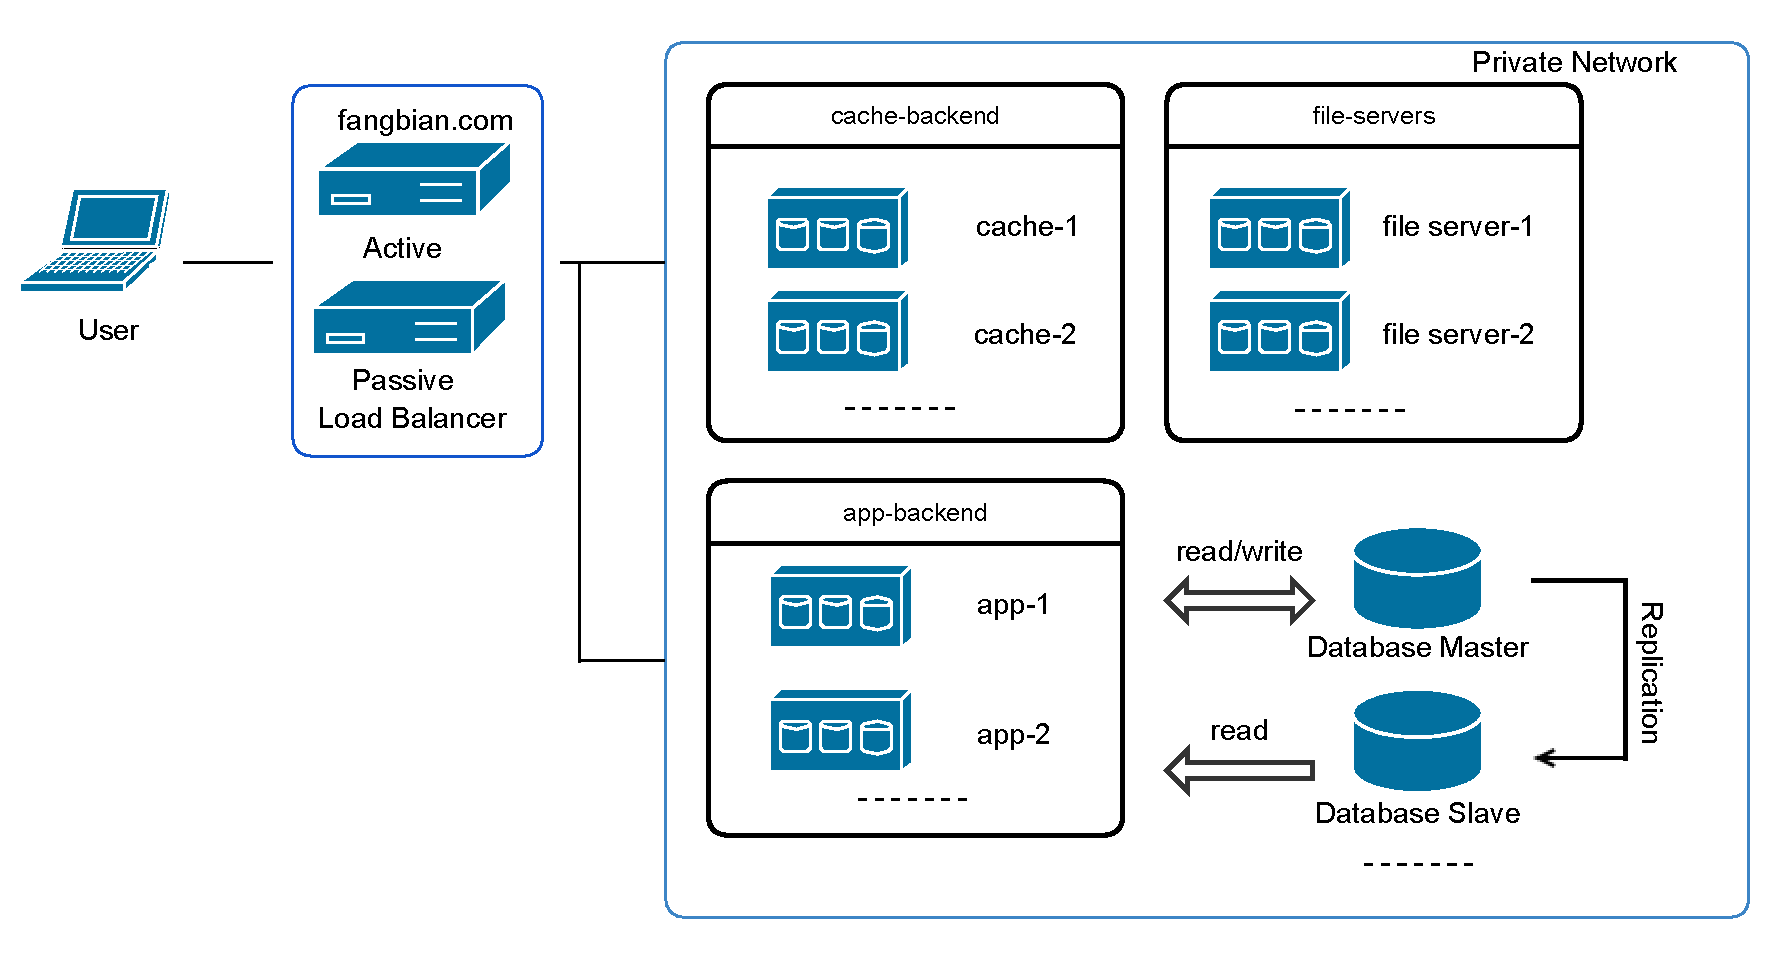
\includegraphics[width=1.0\textwidth]{graphics/diagramsvg.pdf}
	\caption{服务器3-Tier基础设置}
	\label{fig:hs}
\end{figure}

\begin{enumerate}[label=(\alph*)]
   \item 请求动态内容。
     \begin{enumerate}[label=(\arabic*)]
       \item 用户向fangbian.com(load balancer)请求
       \item load balancer向后端应用服务器(app-backend)发出请求
       \item app-backend读取数据库并向load balancer返回内容
       \item load balancer向用户返回请求内容
     \end{enumerate}

   \item 请求静态内容。
     \begin{enumerate}[label=(\arabic*)]
       \item 用户向fangbian.com(load balancer)请求
       \item load balancer从cache-backend检查请求内容是cache-hit还是cache-miss
       \item 如果是cache-hit,向load balancer返回请求内容且跳至第7步;如果是cache-miss,则通过load balancer将请求转到app-backend
       \item app-backend从数据库读取并返回内容到load balancer
       \item load balancer将收到的内容传递到cache-backend 
       \item cache-backend缓存内容然后向load balancer返回内容
       \item load balancer向用户返回请求内容
     \end{enumerate}
\end{enumerate}
\par 提示:设置active/passive负载均衡对(需要虚拟/浮动IP(LVS))可以应对负载均衡失效的问题。例如HAProxy,Nginx等。

\subsection{整体网络架构}
\begin{figure}[H]
	\centering
	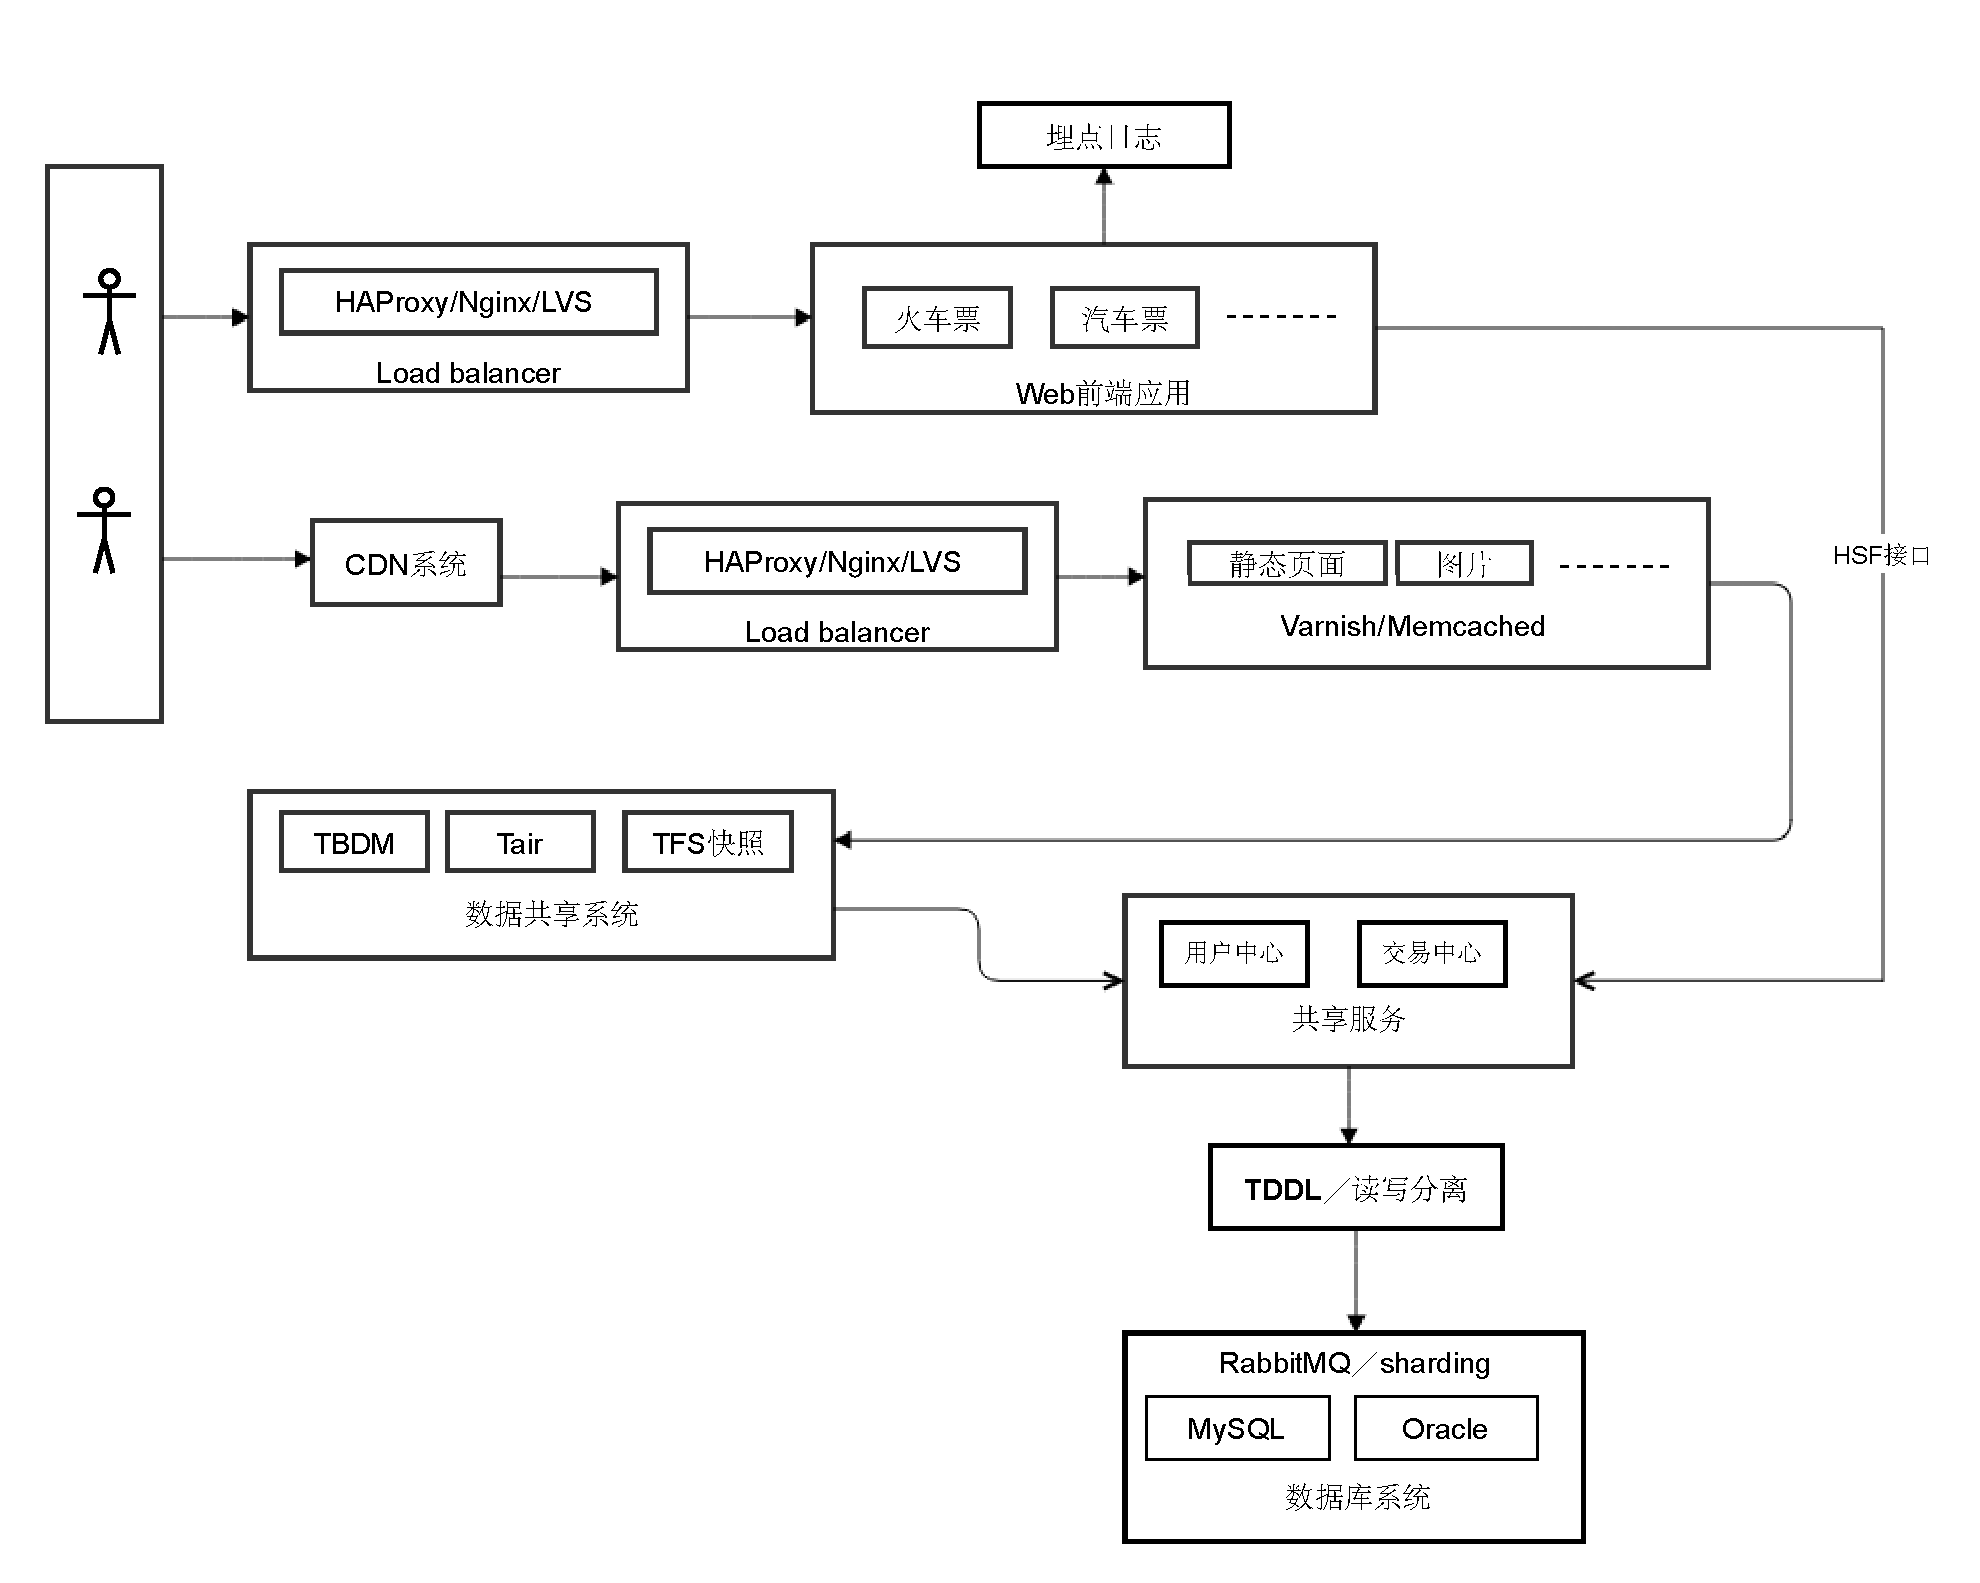
\includegraphics[width=1.0\textwidth]{graphics/tech.pdf}
	\caption{整体网络架构图}
	\label{fig:tech}
\end{figure}


\subsection{分布式架构的服务相关内容}
\begin{figure}[H]
	\centering
	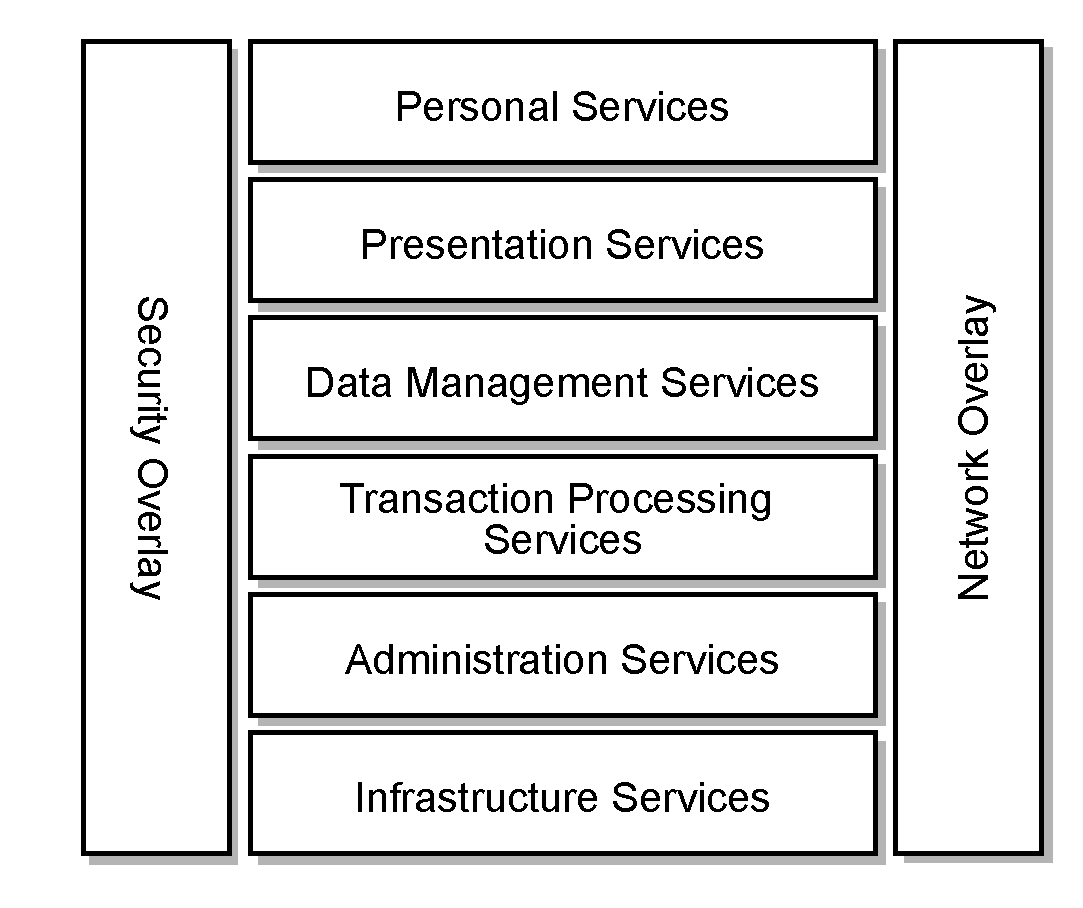
\includegraphics[width=0.7\textwidth]{graphics/architecture.pdf}
	\caption{分布式架构}
	\label{fig:architecture}
\end{figure}

\subsubsection{个人服务}
\begin{enumerate}
   \item 任何基于浏览器的应用。
   \item 建议:
       \begin{enumerate}[label=(\arabic*)]
       \item 坚持标准
       \item 避免使用只针对特定浏览器的特性
       \item 尽量简化逻辑判断
       \item 使用后端语言实现复杂逻辑
     \end{enumerate}
\end{enumerate}

\subsubsection{展现服务}
\begin{enumerate}
   \item 动态内容分发。
   \item 格式化与数据读取。
   \item web组件(例如Portlets)
   \item 建议:
       \begin{enumerate}[label=(\arabic*)]
       \item 数据读取和格式化分离
       \item 业务规则和显示逻辑不能混在一起
       \item 可以参考MVC
     \end{enumerate}
\end{enumerate}

\subsubsection{数据处理服务}
\begin{enumerate}
   \item 搜索。
   \item 分类。
   \item 内容聚合。
   \item 成员协作。
   \item 分配。
   \item 建议:
       \begin{enumerate}[label=(\arabic*)]
       \item 鉴定用户类型;
       \item 关注特定用户类型的目标;
       \item 考虑性能;
       \item 可以参考Chain of Responsibility Patterns和Presentation-Abstraction-Control.
     \end{enumerate}
\end{enumerate}

\subsubsection{交易处理服务}
\begin{enumerate}
   \item 交易管理。
   \item 元数据控制。
   \item 应用接口。
   \item 业务规则。
   \item 数据交换。
   \item 建议:
       \begin{enumerate}[label=(\arabic*)]
       \item 关注接口;
       \item 关注用户未完成的活动;
       \item 不要在业务规则上Hard coding;
       \item 参考observer,Adapter;
     \end{enumerate}
\end{enumerate}

\subsubsection{管理服务}
\begin{enumerate}
   \item LDAP.
   \item 系统管理。
   \item 状态管理。
   \item session管理。
   \item 用户控制。
   \item 规则定义。
   \item 建议:
       \begin{enumerate}[label=(\arabic*)]
       \item 定义策略;
       \item 控制系统状态;
       \item 预估增长;
       \item 参考Command 和 Microkernel;
     \end{enumerate}
\end{enumerate}

\subsubsection{基础设施服务}
\begin{enumerate}
   \item data access.
   \item 通信。
   \item 进程和线程管理。   
   \item 建议:
       \begin{enumerate}[label=(\arabic*)]      
       \item 参考Abstract Factory;
     \end{enumerate}
\end{enumerate}

\subsubsection{安全覆盖层}
\begin{enumerate}
   \item 硬件防火墙.
   \item 软件防火墙。
   \item SSL and WTLS。   
   \item 数据加密。   
   \item 建议:
       \begin{enumerate}[label=(\arabic*)]      
       \item 建立相关策略;
       \item 入侵监视;
       \item patch;
     \end{enumerate}
\end{enumerate}

\subsubsection{网络覆盖层}
\begin{enumerate}
   \item 路由,网关.
   \item 负载均衡。
   \item 建议:
       \begin{enumerate}[label=(\arabic*)]      
       \item 文档,标签,图表;
       \item 将各主要应用分开;
     \end{enumerate}
\end{enumerate}

\subsubsection{集群的监控及管理}
\begin{enumerate}[label=(\alph*)]
   \item 监控:
    \begin{enumerate}[label=(\arabic*)]
      \item Nagios 用来即时监控集群中主机及服务的状态,并给管 理者发送报警信息。
      \item Cacti 记录集群运作中的各种数据,并绘制出图形,为管 理者提供有效的数据支持。
    \end{enumerate}
   \item 管理:
    \begin{enumerate}[label=(\arabic*)]
     \item 如果节点较少,可以基于 ssh + key 编写脚本进行管理。
     \item csync2 也可实现配置文件更改时触发指定脚本的执行。
     \item 较多的节点可以考虑使用 pssh (parallel ssh) 进行管理。
     \item FUNC (Fedora Unified Network Controller) 实现对大量节 点的复杂管理。
    \end{enumerate}
\end{enumerate}

\par 注:应对集群节点可能出现的故障,可以使用keepalived\footnotemark[1]来解决。
\fancyfootnotetext{1}{\urlstyle{sf} \url{http://www.keepalived.org/}}

% \par 静态文件,用Varnish缓存
% \par 对数据库查询的数据,使用Memcached。
% \par 容灾:赛门铁克,爱数
% \par MySQL sharding 

\section{fangbian.com网络架构}

\subsection{fangbian.com网络架构介绍}
\par 方便网网络架构
\begin{figure}[H]
	\centering
	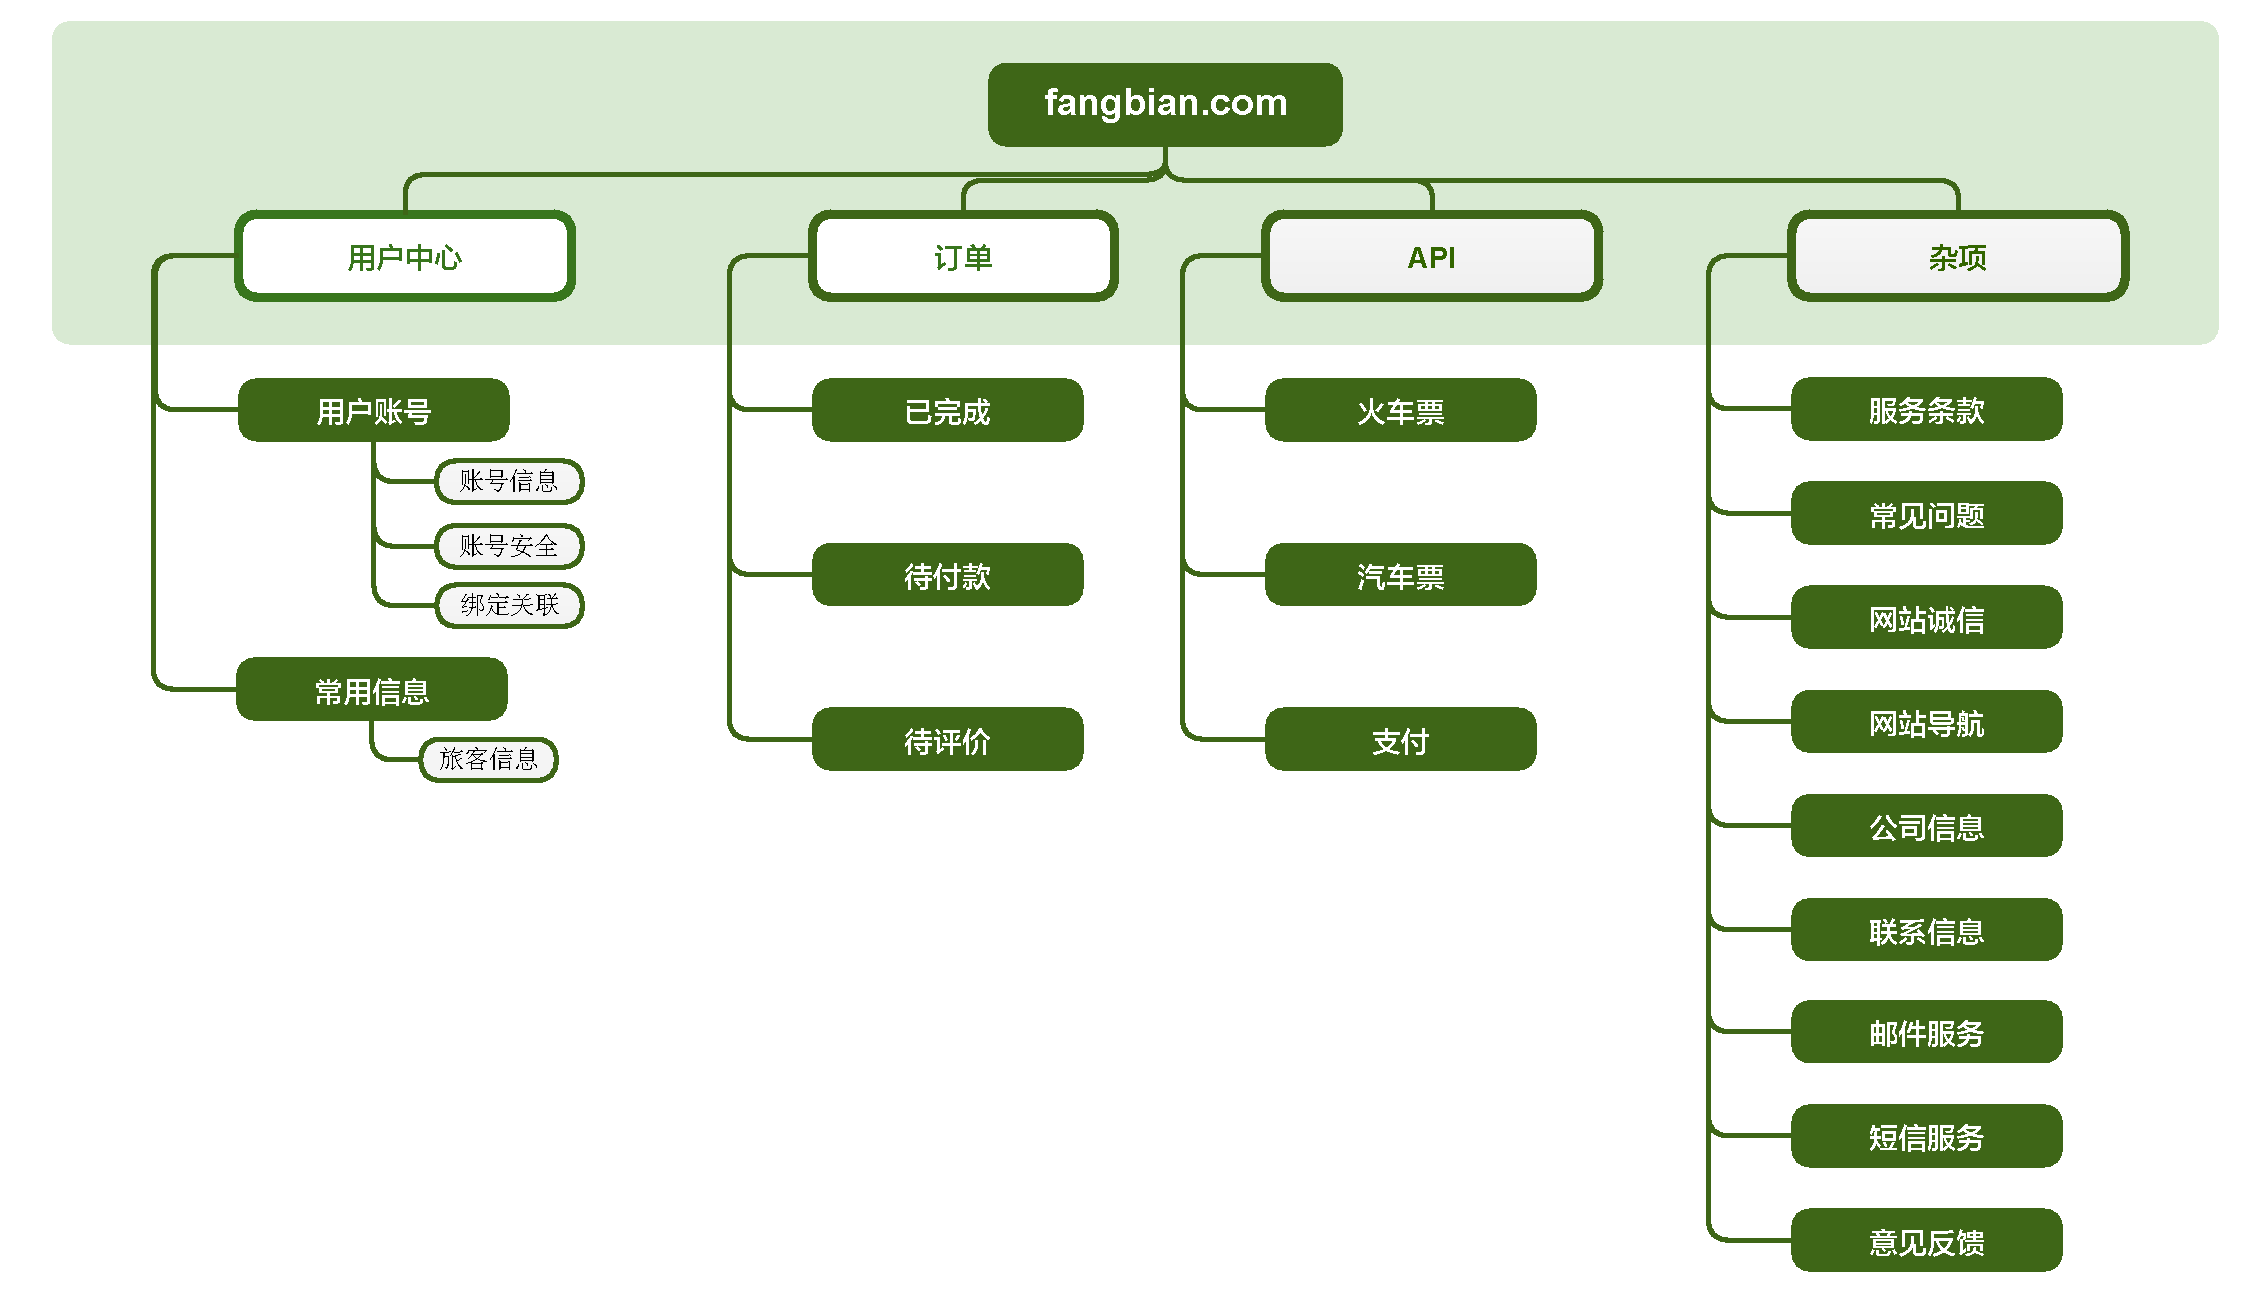
\includegraphics[width=1.0\textwidth]{graphics/fangbian.pdf}
	\caption{方便网网络架构}
	\label{fig:fb}
\end{figure}

\par 图表内容主要是基于现有的两项业务。

% \par 可以引入中间件\footnotemark[1]
% \fancyfootnotetext{1}{this is the footnote}


\section{开发workflow}

\subsection{git workflow}
\par 方便网开发的workflow
\begin{figure}[H]
	\centering
	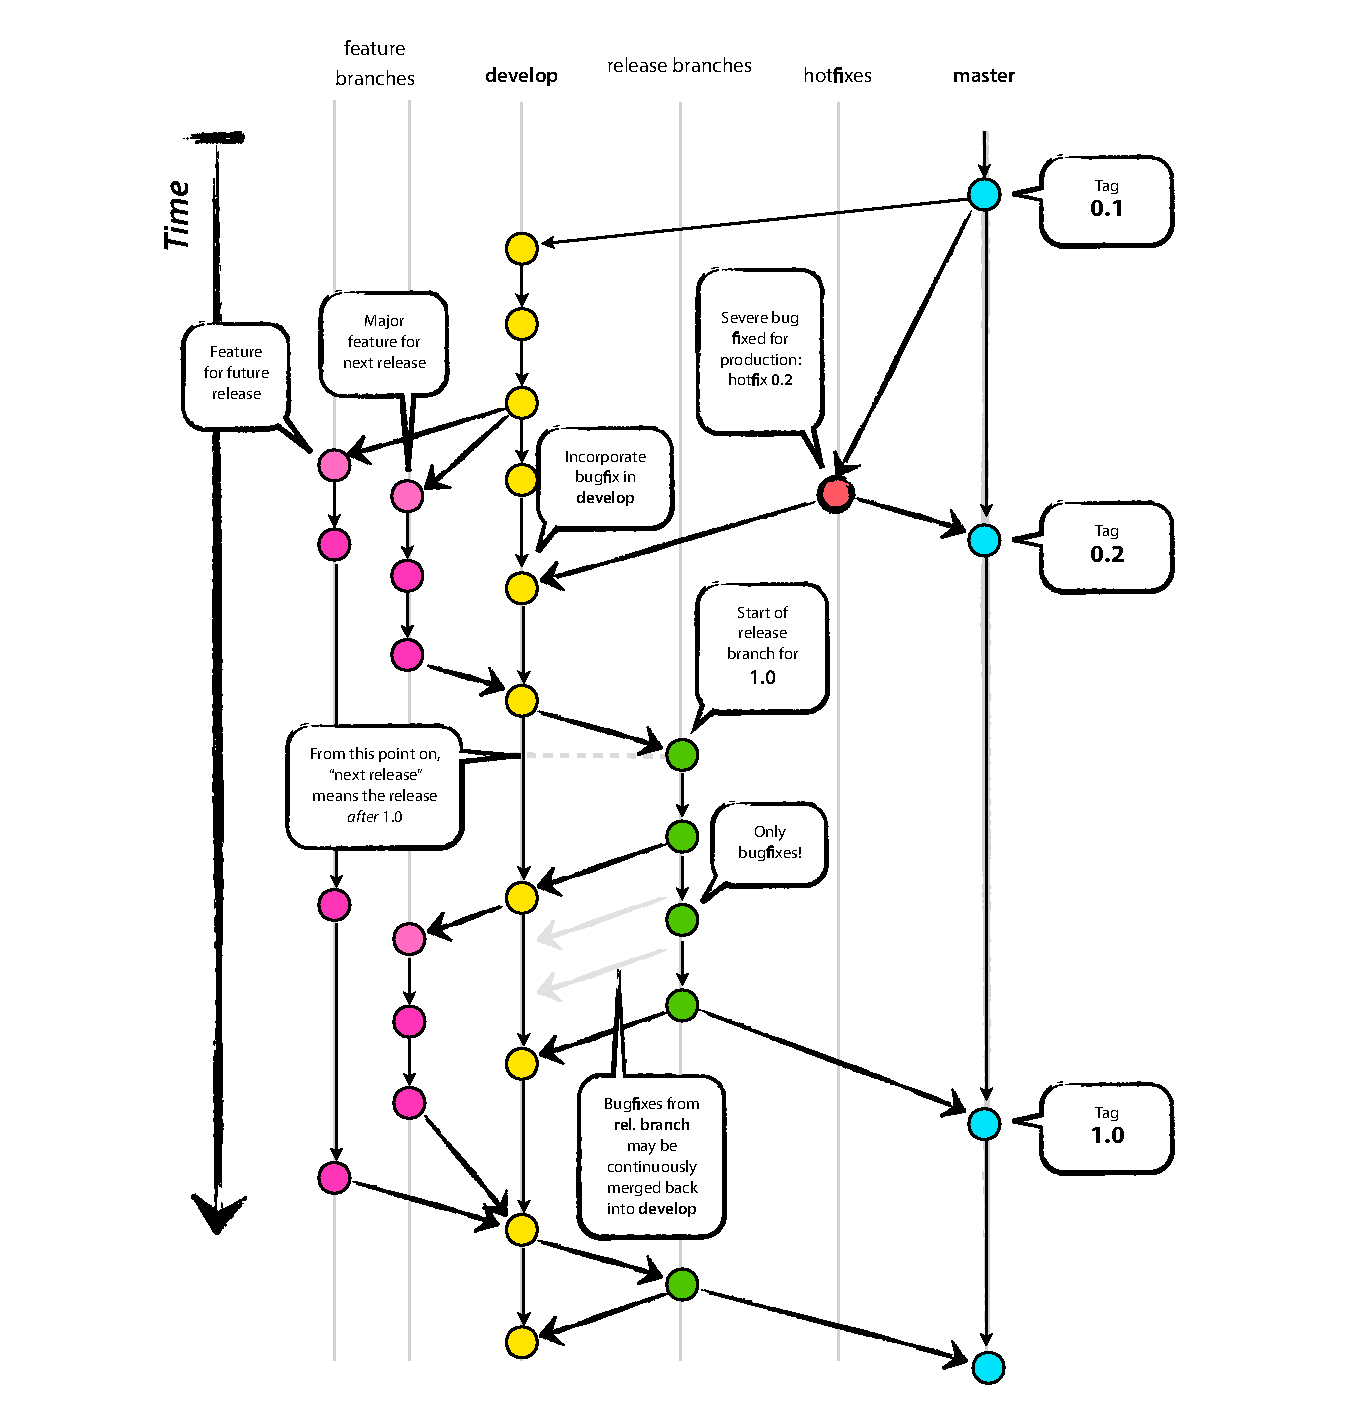
\includegraphics[width=1.0\textwidth]{graphics/gitflow-model.pdf}
	% \caption{\footnotemark[2]}
	\caption[Caption for LOF]{git workflow\protect\footnotemark[1]}
	\label{fig:gitflow}
\end{figure}
\fancyfootnotetext{1}{原作者:Vincent Driessen 地址:http://nvie.com/posts/a-successful-git-branching-model/ 本文稍作修改。}

\subsection{开发规范}
\par 以前端开发规范为例:
\begin{enumerate}[label=(\arabic*)]
    \item 代码规范,\urlstyle{sf} \url{http://google-styleguide.googlecode.com/svn/trunk/};
    \item 目录结构,js、images、css(less/sass),test目录文件结构;
    \item js库依赖,bower;
    \item 使用sass,less、coffeescript,jade等需要编译的文件,即时编译;
    \item UI库(sprites、js的类,常见的,popup,tab,slider,tip等等);
    \item 版本管理,git;
    \item js、css压缩合并,grunt,gulp等;
    \item wiki: MediaWiki;  
    \item bug管理: bugzilla;    
    \item 防止缓存:grunt;
    \item Unit test,e2e测试,集成测试;      
    \item 安全,最常见的是XSS和CSRF。
\end{enumerate}

\fancyfootnotetext{1}{本文源代码地址:}

% \input{./partials/chapter05.tex}

\end{document}
